\documentclass[10pt,aspectratio=1609]{beamer}
\usepackage{hyperref}
\usepackage{amsmath}

% \usetheme{CambridgeUS}
\usepackage{aneotheme}


\begin{document}
\author{Jérôme Gurhem}
\title{Cloud computing with \\ ArmoniK}
\subtitle{CSMA Juniors 2025}
\institute{Aneo}
\date{\today}

\titlepage

\AtBeginSection[]
{
	\frame{\sectionpage}
}

\begin{frame}
	\frametitle{Outline}
	\large
	\tableofcontents
\end{frame}

\begin{section}{Our expertise @Aneo}
  \begin{frame}
    \frametitle{Who are we ?}
    \begin{itemize}
      \item Consulting agency specialized in digital transformation
      \item Support for organizational transformations
      \item Assistance in carrying out advanced IT projects
      \item 150 employees
      \item HPC/HTC R\&D team of $\sim$30 people, including 15 PhDs
    \end{itemize}
  \end{frame}

  \begin{frame}
    \frametitle{Technical expertise}
    \begin{itemize}
      \item Code optimization
      \begin{itemize}
        \item Performance analysis and bottleneck identification
        \item Porting applications to support GPU
        \item Application industrialisation (automation, reliability, repeatability)
      \end{itemize}
      \item Cloud computing
      \begin{itemize}
        \item Application migration to a specific cloud provider (AWS, GCP or Azure)
      \end{itemize}
      \item ArmoniK
      \begin{itemize}
        \item Links our expertise domains
      \end{itemize}
      \item Numerical instabilities detection
      \begin{itemize}
        \item InterFLOP
      \end{itemize}
    \end{itemize}
  \end{frame}

  \begin{frame}
    \frametitle{Floating Point Arithmetic}
    \begin{itemize}
      \item Interflop ANR project with:Aneo, CEA - LIST, EDF, Intel, Sorbonne Université - LIP6, Triscale-Innov, Université Perpignan - LAMPS, UVSQ - Li-PaRAD
      \item Analyzing round-off error propagation in numerical applications
      \item ANEO's contribution:
      \begin{itemize}
        \item Development of PENE
        \item Stochastic Arithmetic: modification of rounding errors in every FP operation
        \item Delta Debug: locate the source of the instabilities in the source code
        \item Dynamic Compilation: based on Intel PIN
        \item Portability: x86 on Linux and Windows
      \end{itemize}
    \end{itemize}
  \end{frame}
\end{section}

\begin{section}{Our vision of Cloud Computing}
  \begin{frame}
    \frametitle{What is the Cloud?}
      \begin{alertblock}{Definition}
      \begin{quote}
        Paradigm for enabling network access to a scalable and elastic pool of shareable physical
        or virtual resources with self-service provisioning and administration on-demand.
        \\
        --- ISO/IEC 17788:2014
      \end{quote}
    \end{alertblock}
  \end{frame}

  \begin{frame}
    \frametitle{Fundamental Principles}
    \centering
    \vfill
    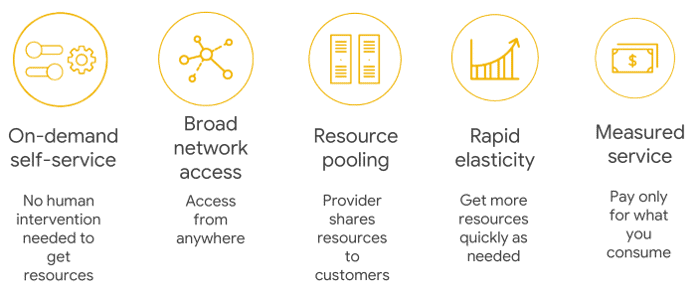
\includegraphics[width=\textwidth]{cloud-fundamentals.png}
  \end{frame}

\begin{frame}
  \frametitle{Cloud Deployment Models}

  \begin{itemize}
    \item \textbf{Public Cloud}
    \begin{itemize}
      \item Resources are owned and operated by a third-party provider (e.g., AWS, Azure)
      \item Shared infrastructure across multiple customers
    \end{itemize}

    \item \textbf{Private Cloud}
    \begin{itemize}
      \item Cloud infrastructure dedicated to a single organization
      \item Hosted on-premises or by a third party
    \end{itemize}

    \item \textbf{Hybrid Cloud}
    \begin{itemize}
      \item Combines public and private clouds
      \item Allows data and apps to move between environments
    \end{itemize}
  \end{itemize}
\end{frame}

\begin{frame}
  \frametitle{Cloud Service Models}

  \begin{itemize}
    \item \textbf{Infrastructure as a Service (IaaS)}
    \begin{itemize}
      \item Provides virtual machines, networking, and storage
      \item User manages OS, apps, and runtime
      \item \emph{Example: Amazon EC2, Google Compute Engine}
    \end{itemize}

    \item \textbf{Platform as a Service (PaaS)}
    \begin{itemize}
      \item Provides platforms to develop, run, and manage applications
      \item Abstracts infrastructure management
      \item \emph{Example: Heroku, Google App Engine}
    \end{itemize}

    \item \textbf{Software as a Service (SaaS)}
    \begin{itemize}
      \item Delivers software over the internet
      \item User only interacts with the application
      \item \emph{Example: Gmail, Dropbox, Salesforce}
    \end{itemize}

    \item \textbf{Serverless}
    \begin{itemize}
      \item Application infrastructure tends to be abstracted away
      \item Same goes for computing resources
    \end{itemize}
  \end{itemize}
\end{frame}

\begin{frame}
  \frametitle{Scale of Computations}

  \begin{columns}[T] % Align columns at the top
    \begin{column}{0.33\textwidth}
      \textbf{Large scale computations}
      \begin{itemize}
        \item 100s of nodes
        \item Tight coupling
        \item Need for low latency network for good performance
        \item Based on MPI+X
      \end{itemize}
    \end{column}
    \begin{column}{0.33\textwidth}
      \textbf{Medium scale computations}
      \begin{itemize}
        \item Tend to fit on 1 node with 100s of cores
        \item Previously based on MPI+X
        \item No longer needed due to single node performance
        \item Possible need for parametric study
      \end{itemize}
    \end{column}
    \begin{column}{0.33\textwidth}
      \textbf{Small scale computations}
      \begin{itemize}
        \item Fit on developers' laptop
        \item Possible need for parametric study
      \end{itemize}
    \end{column}
  \end{columns}

  % \vspace{1cm}
  % \centering
  % \begin{tikzpicture}[remember picture]
  %   \draw[aneoorange, ->, ultra thick]
  %     ([xshift=0.2\textwidth]current page.west) --
  %     ([xshift=-0.2\textwidth]current page.east)
  %     node[midway, below] {Technical evolution};
  % \end{tikzpicture}
\end{frame}

\begin{frame}
  % todo: verify this slide
  % ethernet should be checked
  \frametitle{Large Scale Computations}

  \begin{itemize}
    \item \textbf{On-premises}
    \begin{itemize}
      \item SLURM, Torque, Moab
      \item HPC clusters / supercomputers
      \item High-speed interconnects (InfiniBand, Omni-Path)
    \end{itemize}

    \item \textbf{Amazon Web Services (AWS)}
    \begin{itemize}
      \item Managed services : AWS Batch, AWS ParallelCluster (SLURM)
      \item Colocated resources with high-speed ethernet (Elastic Fabric Adapter from AWS)
      \item Limited to the configurations exposed by AWS
      \item Useful to start quickly
    \end{itemize}

    \item \textbf{Google Cloud Platform (GCP)}
    \begin{itemize}
      \item Managed service : Google Batch
      \item Colocated resources with high-speed ethernet (Google Cloud's high-speed network)
      \item Aneo contributes on High Availability for GCP SLURM deployment available in Cluster Toolkit
      \item More configuration options but should be deployed by the user (vs managed services)
    \end{itemize}
  \end{itemize}
\end{frame}


\begin{frame}
  \frametitle{Medium/Small Scale Computations}

  \begin{itemize}
    \item \textbf{1rst Game changers: Power of 1 node}
    \begin{itemize}
      \item NVidia H series GPU for 67 TFLOPS in FP64 and 4 PFLOPS in FP8 on tensor cores
      (\href{https://nvdam.widen.net/s/nb5zzzsjdf/hpc-datasheet-sc23-h200-datasheet-3002446}{datasheet})
      \item AMD EPYC 9965 with 192 cores and 384 threads (bi-processor)
    \end{itemize}

    \item \textbf{2nd Game changers: Cloud Providers}
    \begin{itemize}
      \item Very expensive powerful nodes
      \item Available on-demand and pay-as-you-go on the Cloud
      \item Affordable to use them for small/medium scale computations
    \end{itemize}

    \item \textbf{Impacts}
    \begin{itemize}
      \item Applications running on a few nodes can now run on a single node
      \item Buying powerful nodes without fully using them is not whorth it
      \item Better rent them only when needed
    \end{itemize}

    \item \textbf{3nd Game changers: Parametric studies}
    \begin{itemize}
      \item Small unitary runs
      \item Needs a lot of them for exploring the parameter space or for Monte-Carlo simulations
      \item Pre-processing and post-processing of potentially different nature and machines requirements
      \item Need for integration of AI steps to accelerate exploration
      \item May be large scale computations at the end
    \end{itemize}

  \end{itemize}
\end{frame}

\begin{frame}
  \frametitle{Recap}

  \begin{itemize}
    \item Computations nature is changing with AIs and hardware evolutions
    \item Cloud introduces new computing paradigms for computations and hardware accessibility
    \item Decoupling of application and infrastructure lead to Serverless computing

    

  \end{itemize}
\end{frame}


\end{section}


\begin{section}{Why we built our own cloud-native scheduler ?}

  \begin{frame}
    \frametitle{Genesis of ArmoniK}
    \begin{itemize}
      \item Multiple task/job schedulers and orchestrators already exist in the market.
      \item Each has unique properties and programming paradigms tailored to different use cases.
      \item However, none of these solutions offered all the features we required for our specific needs.
      \item Aneo has experience working with both commercial and private task scheduling systems, providing valuable
      insights into the gaps and limitations.
      \item We’ve contributed by implementing missing features or developing workarounds to address the gaps in
      existing systems.
      \item A significant amount of effort has been spent solving the same challenges across various systems.
      \item We identified an opportunity to build our own solution that is tailored to our clients’ needs and provides the
      full functionality required.
    \end{itemize}
  \end{frame}

  \begin{frame}
    \frametitle{Opportunity: replace legacy HTC schedulers in Finance}
    \begin{itemize}
      \item Since early 2000's, market is shared between two proprietary software (IBM Symphony and Tibco Datasynapse)
      \item Algorithms in finance were simple: Monte-Carlo is well suited for HTC
      \item Since 2008, market regulators have enforced an evolution in the algorithms
      \begin{itemize}
        \item Sensitivity to the risk factors
        \item Bank-level vs portfolio-level risk computation
        \item Calibration must be mutualized between assets
        \item Volatility calibration is much more expensive
      \end{itemize}
    \end{itemize}
    
    $\Rightarrow$ Integrating the compute library with the scheduler becomes more and more complex
  \end{frame}


  \begin{frame}
    \frametitle{2020: a partnership with Crédit Agricole (CACIB) and AWS}
    \begin{columns}
      \column{0.5\textwidth}
      \begin{itemize}
        \item ANEO is responsible to develop a new open-source solution that
        \begin{itemize}
          \item Replaces all schedulers used by CACIB
          \item Provides the same level of performances as proprietary solutions
          \item Is portable on-prem/cloud (AWS, GCP, Qarnot, OVH)
          \item Is elastic and autoscalable
          \item Is portable Linux/Windows
          \item Is usable in many languages (e.g.: C\#, Java, C++, Python)
        \end{itemize}
      \end{itemize}
      \column{0.5\textwidth}
      \begin{itemize}
        \item The solution must be in production mid-2022
        \begin{itemize}
          \item Native observability
          \item Fault-tolerance
        \end{itemize}
        \item ANEO adds some requirements
        \begin{itemize}
          \item Leverage Task-based programming
          \item Allow for dynamic graphs
          \item Industrialize the users' development process
          \item Transfer HPC know-how into new fields
        \end{itemize}
      \end{itemize}
    \end{columns}
  \end{frame}
  
  \begin{frame}
    \frametitle{ArmoniK: a Hybrid Framework}
    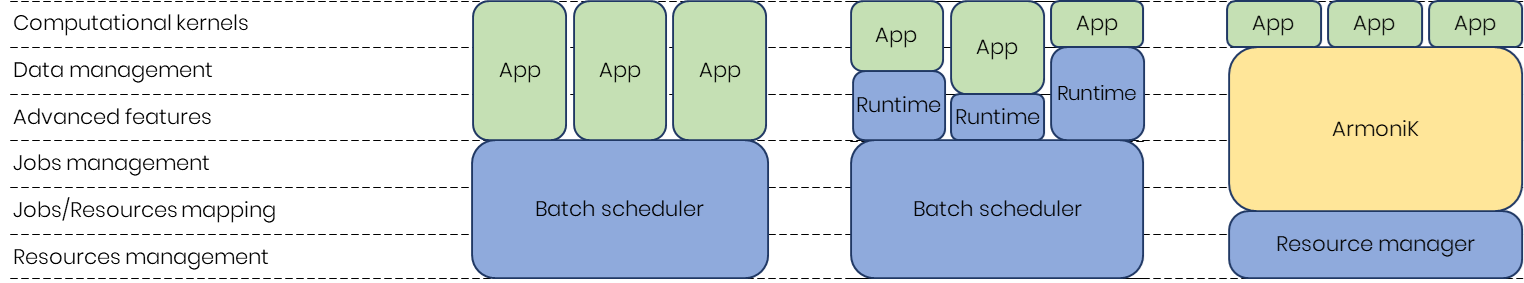
\includegraphics[width=\textwidth]{hpc-orchestrators.png}
    \begin{itemize}
      \item Computational kernels: User computations
      \item Data management: Reads, Writes, Communications between processes
      \item Advanced features: Overlapping, load balancing
      \item Jobs management: Job queues, resource allocation, job lifecycle
      \item Jobs / Resources mapping: Determine job execution on which machines
      \item Resources management: Machine pool update, node addition or removal
    \end{itemize}
  \end{frame}

  \begin{frame}
    \frametitle{Comparison with other schedulers}
    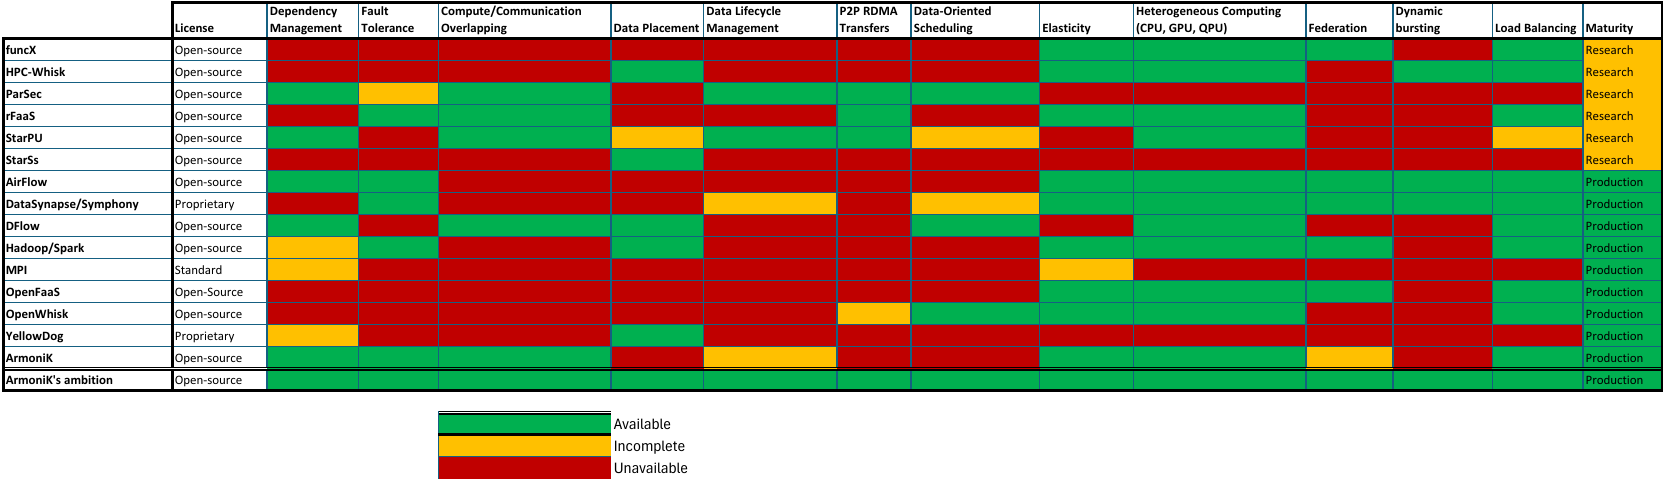
\includegraphics[width=\textwidth]{pos-1.png}
  \end{frame}
\end{section}

\begin{section}{ArmoniK, an answer to ease resilient large scale cloud computing}
  \begin{frame}
    \frametitle{A Serverless Many-Task Computing Ecosystem}
    \begin{alertblock}{Serverless}
      \begin{quote}
        Cloud service category in which the customer can use different cloud capabilities types
        without the customer having to provision, deploy and manage either hardware or software
        resources, other than providing customer application code or providing customer data.
        \\
        --- ISO 22123-2:2023
      \end{quote}
    \end{alertblock}
    \begin{alertblock}{Many-Task Computing}
      \begin{quote}
        Approach that aims to bridge the gap between High-Perfomance Computing and High-Throughput Computing.
        \\
        --- Wikipedia
      \end{quote}
    \end{alertblock}
    \begin{alertblock}{Ecosystem}
      \begin{quote}
        System that environments and their organisms form through their interaction.
        \\
        --- Principles of Terrestrial Ecosystem Ecology, F. Stuart Chapin
      \end{quote}
    \end{alertblock}
  \end{frame}

  \begin{frame}
    \frametitle{Task-based Programming in ArmoniK}
    \begin{block}{Definition}
      Paradigm focusing on the decomposition of complex operations into smaller tasks
    \end{block}
    \begin{itemize}
      \item Expression of complex data-driven dependencies
      \item ArmoniK's \textbf{distributed scheduler} responsible for:
      \begin{itemize}
        \item Task distribution and load balancing
        \item Dependency resolution
        \item Tasks execution
        \item Data management (overlapping, prefetching, and checkpointing)
      \end{itemize}
    \end{itemize}
  \end{frame}

  \begin{frame}
    \frametitle{ArmoniK Programming Model}
    \begin{columns}[T]
      \begin{column}{0.5\textwidth}
        \begin{itemize}
          \item \textbf{Task Graph}: Bipartite DAG whose node sets are tasks and data
          \item \textbf{Task node}: Single-node computation (possibly multi-threaded) taking one or several data inputs and outputting one or several data
          \item \textbf{Data node}: Immutable piece of data depending on only one task at most
          \item \textbf{Dependencies}: Dependencies between tasks are expressed as data dependencies
          \item \textbf{Dynamic}: The graph may not be entirely known in advance (tasks can append tasks and replace edges with subgraphs)
        \end{itemize}
      \end{column}
      \begin{column}{0.5\textwidth}
        \centering
        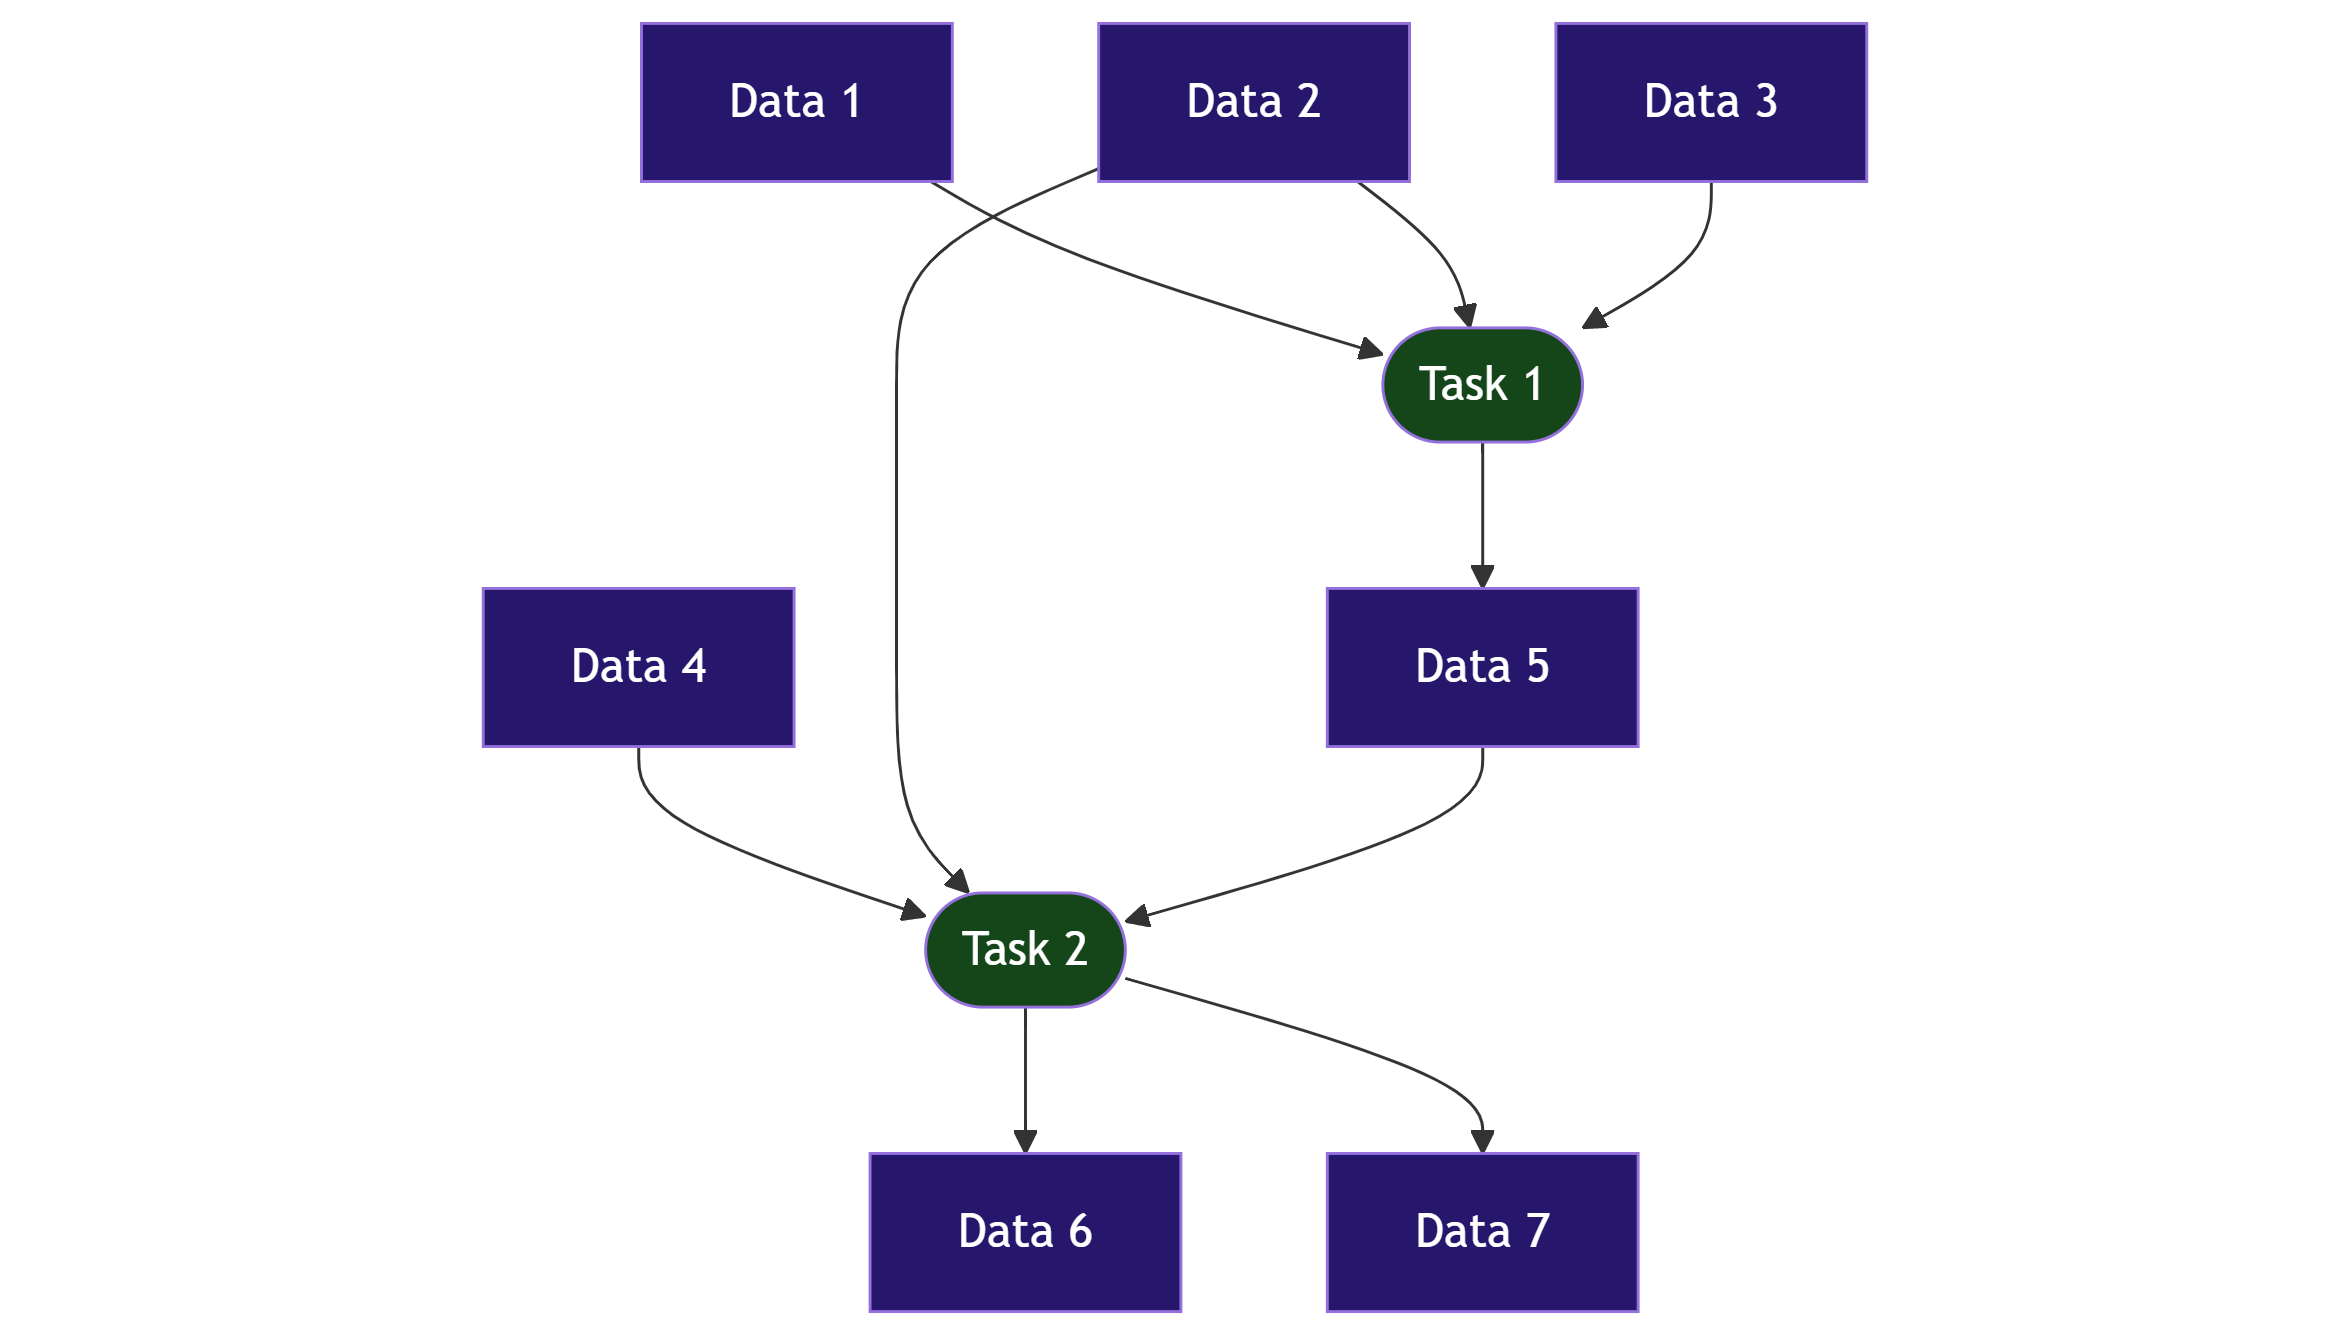
\includegraphics[width=0.95\textwidth]{mermaid-task-graph.png}
      \end{column}
    \end{columns}
  \end{frame}

  \begin{frame}
    \frametitle{The Client-Worker Pattern}
    \begin{columns}[T]
      \begin{column}{0.5\textwidth}
        \begin{itemize}
          \item \textbf{Client}: User-developed software that submits the initial task graphs to ArmoniK and retrieves results
          \item \textbf{Worker}: User-developed software capable of performing one or several tasks, depending on its implementation:
          \begin{itemize}
            \item Can take input data, perform calculations, and return a result
            \item Can submit new tasks and set the result as output of a new task
          \end{itemize}
          \item \textbf{Synchronization via Data}: The client might not be aware that the task graph has been modified
        \end{itemize}
      \end{column}
      \begin{column}{0.5\textwidth}
        \centering
        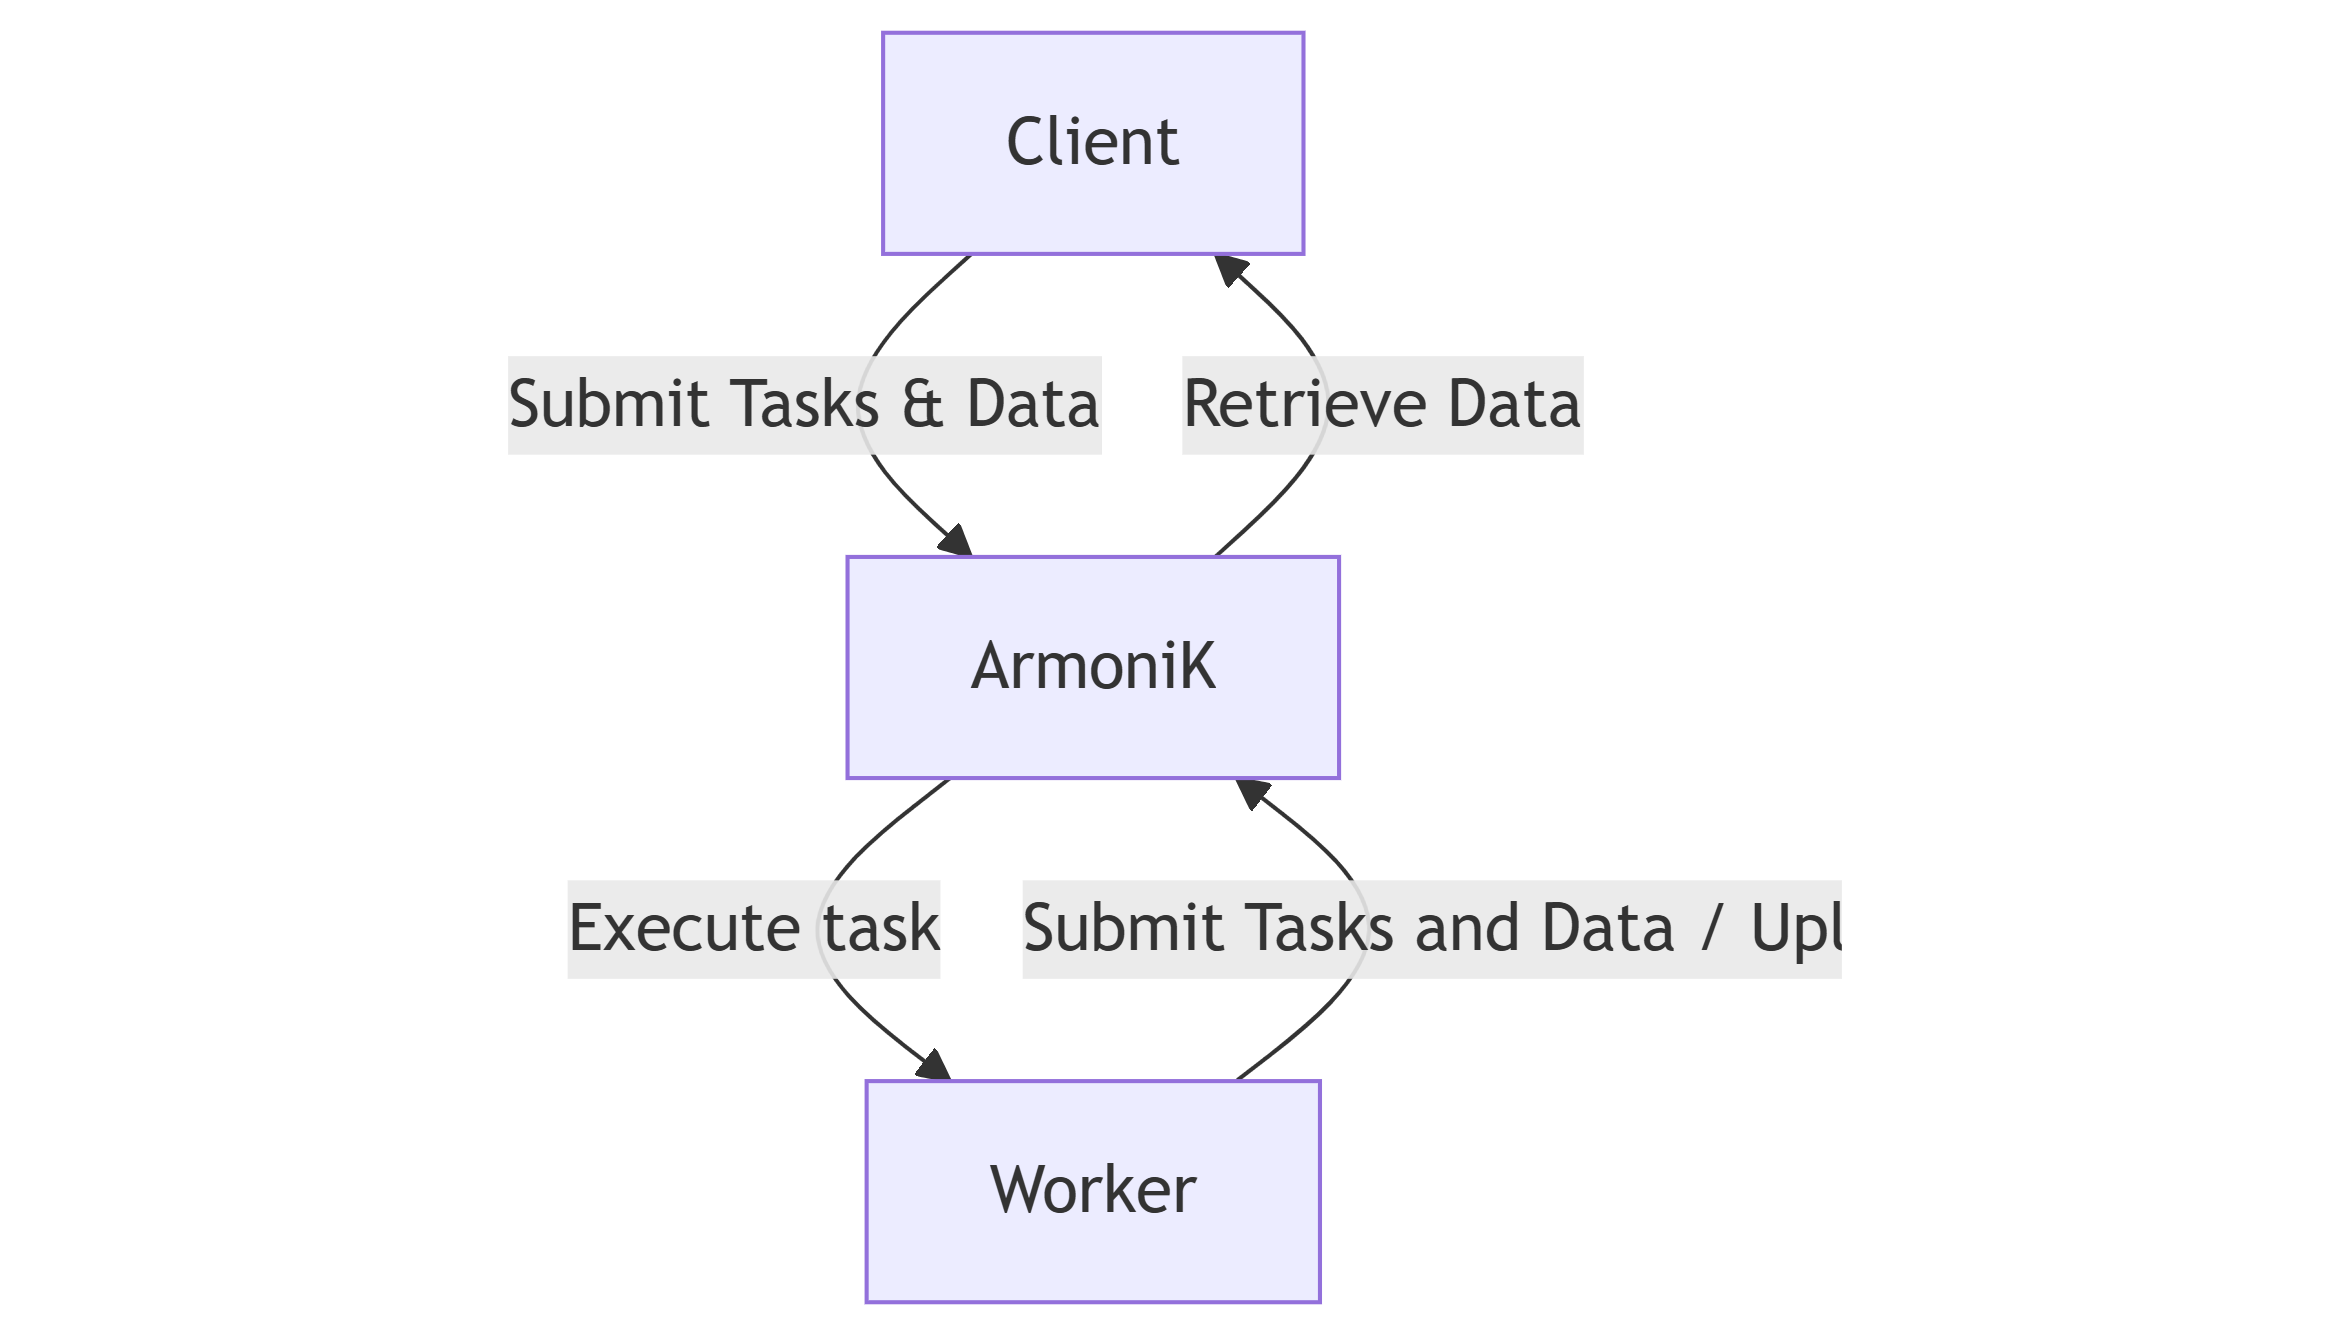
\includegraphics[width=0.95\textwidth]{mermaid-client-worker.png}
      \end{column}
    \end{columns}
  \end{frame}

  \begin{frame}
    \frametitle{Simplified Architecture}
    \centering
    \vfill
    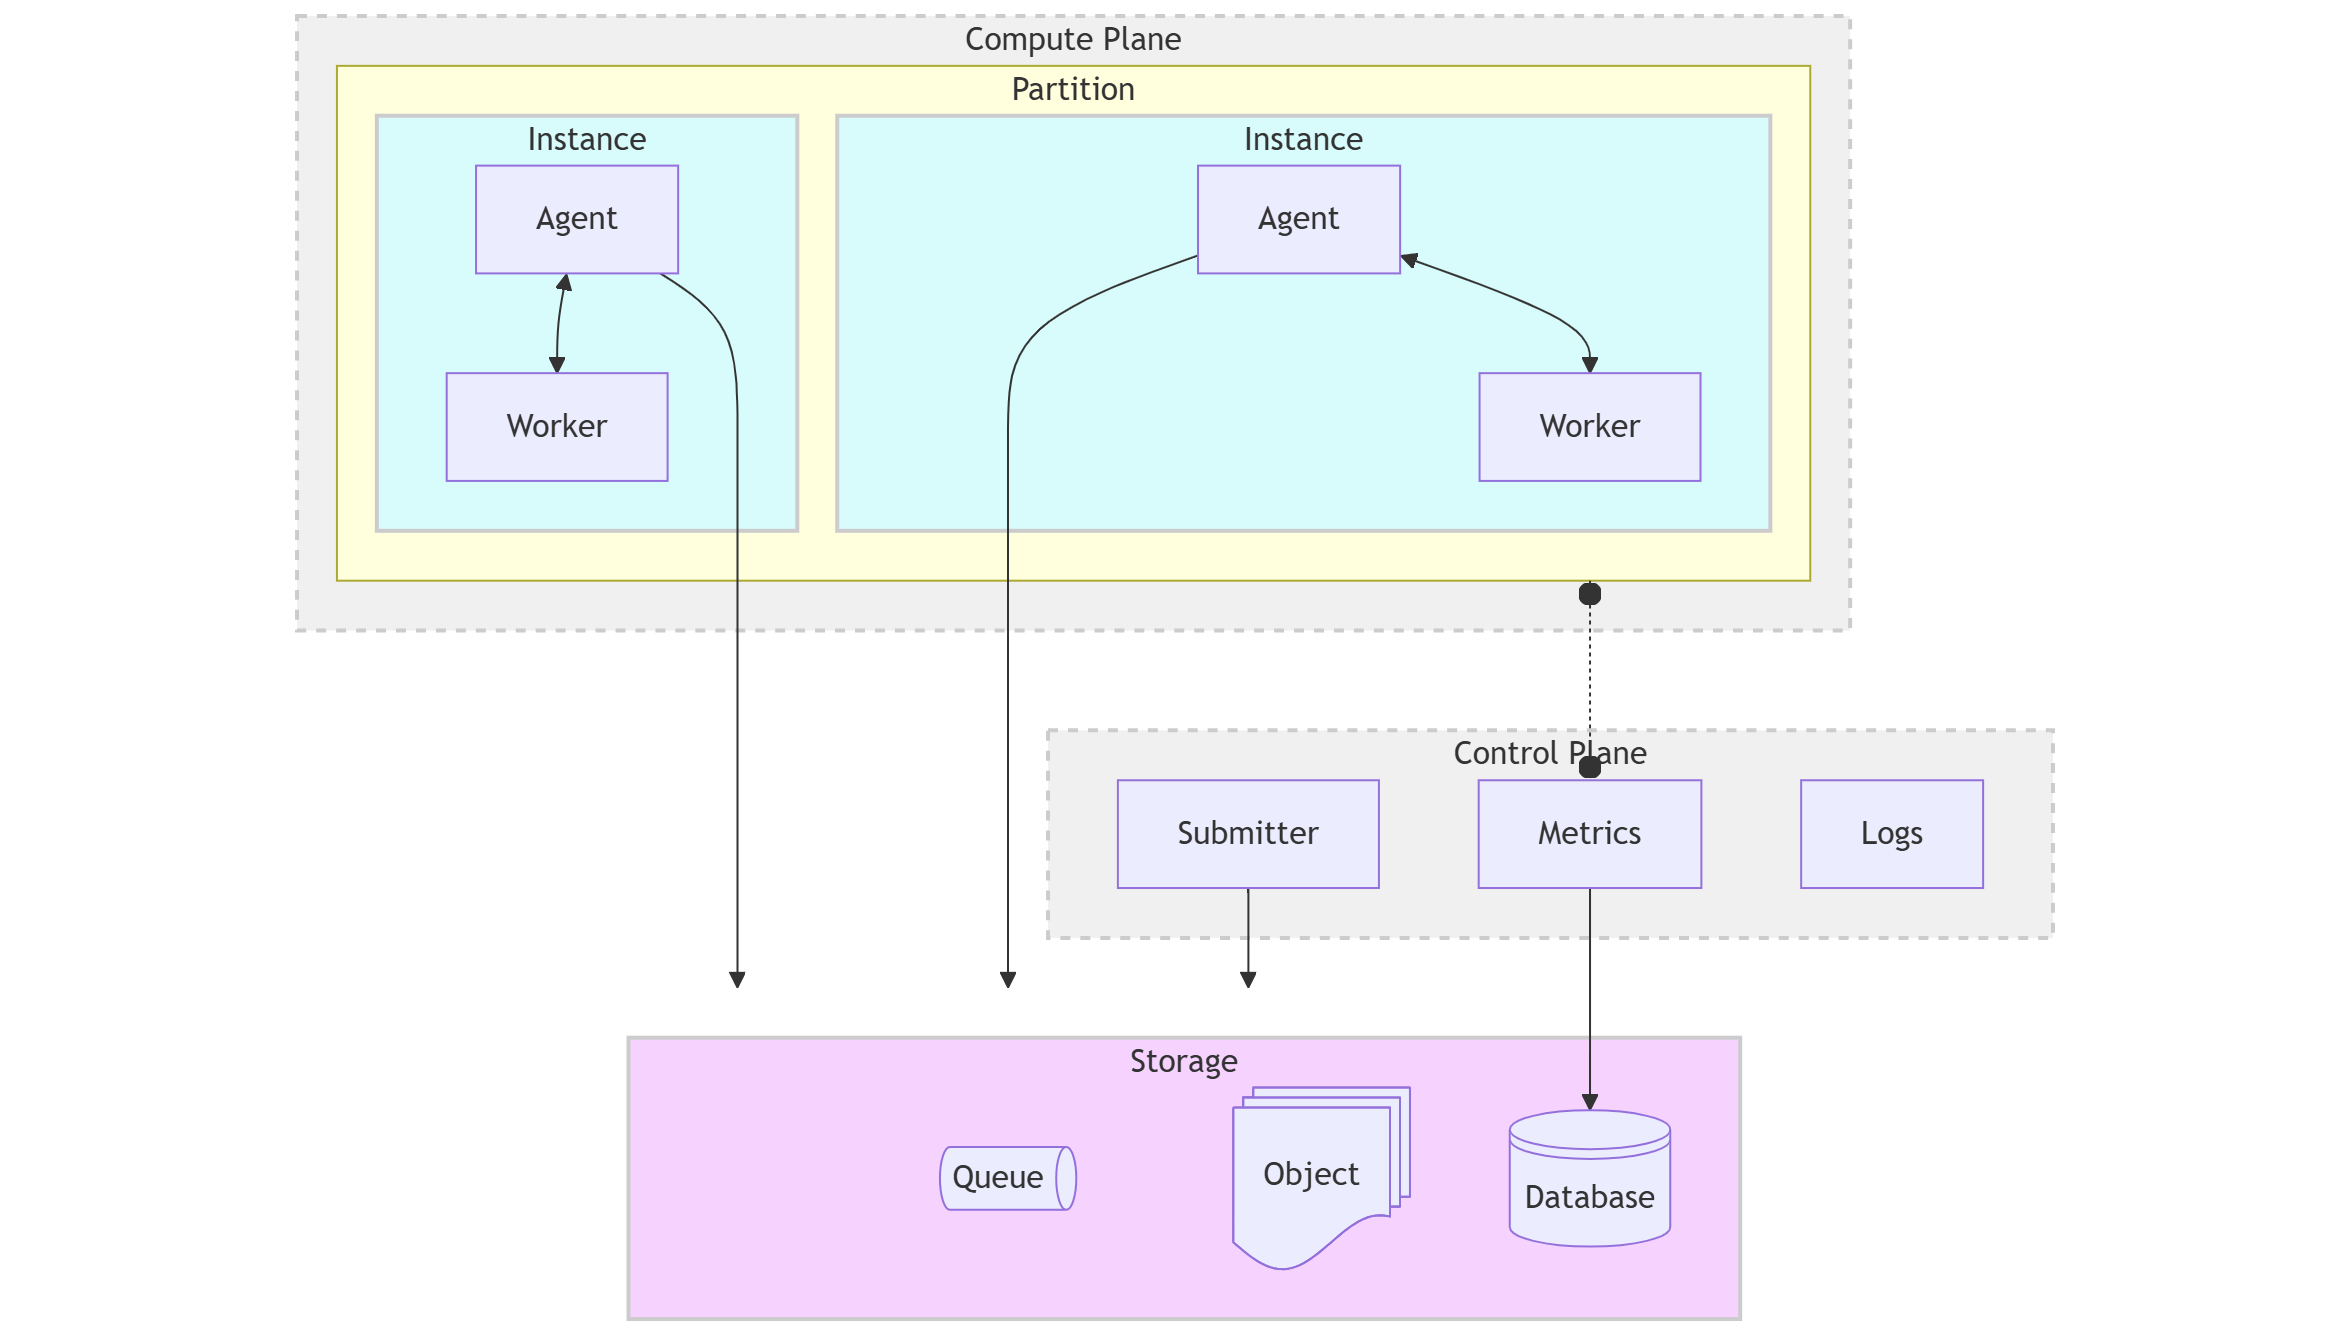
\includegraphics[width=0.95\textwidth]{mermaid-simplifed-architecture.png}
  \end{frame}

  \begin{frame}
    \frametitle{Tasks and Data Processing Cycle in ArmoniK}
    \centering
    \vfill
    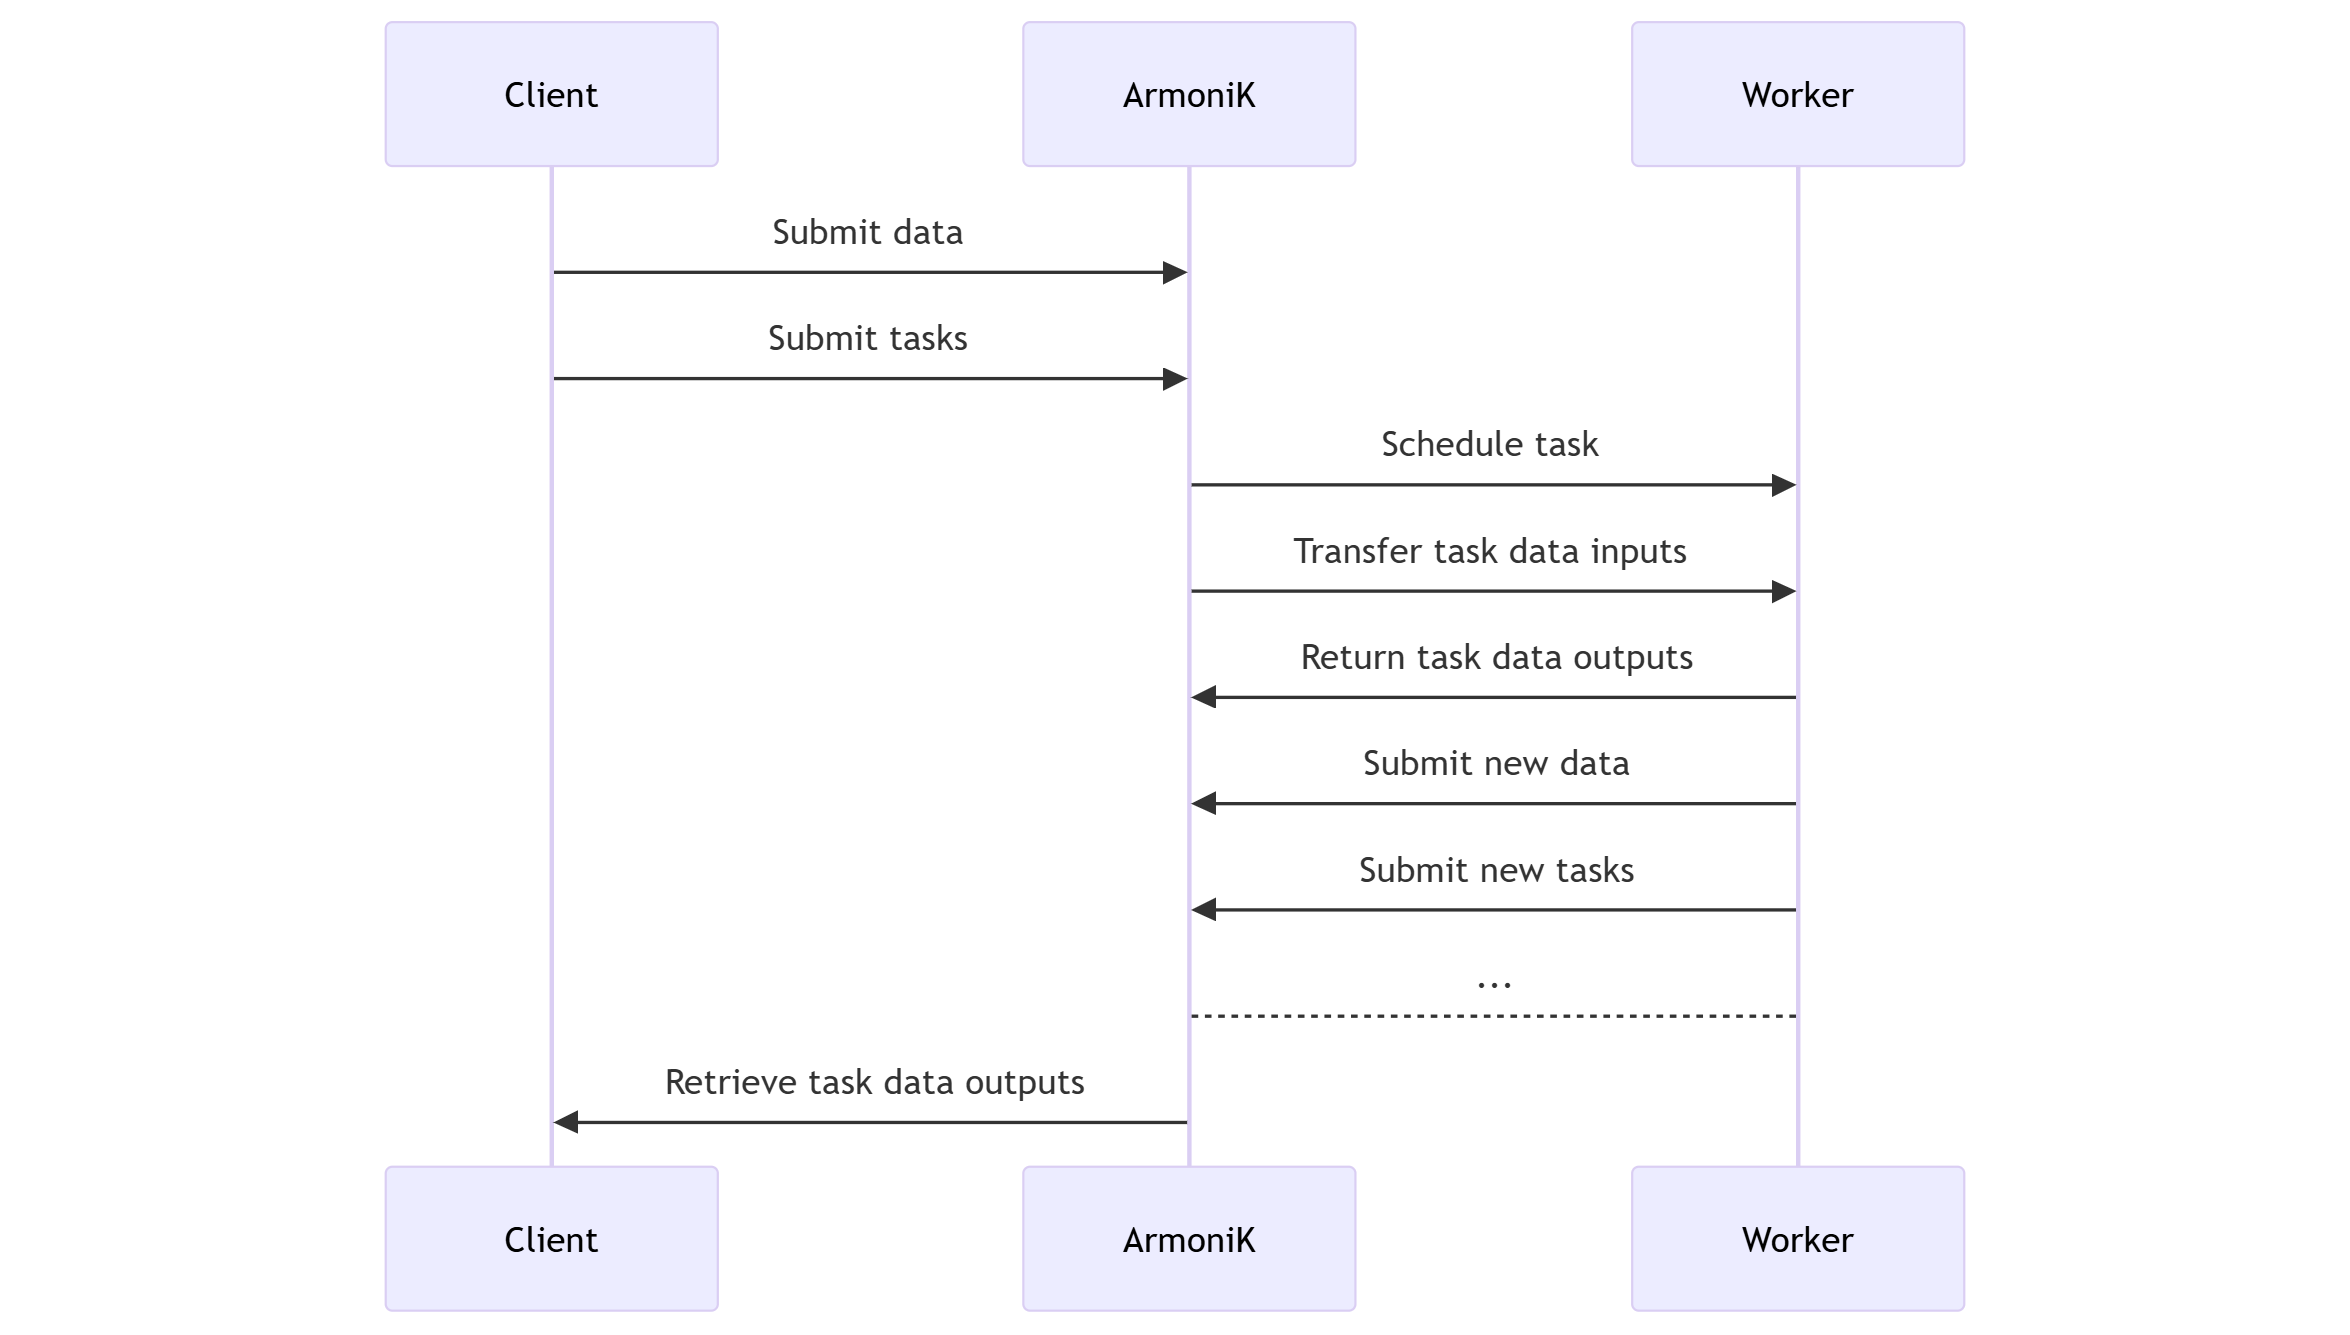
\includegraphics[width=0.95\textwidth]{mermaid-sequence.png}
  \end{frame}

  \begin{frame}
    \frametitle{Dynamic Graph}
    \begin{block}{Definition}
      Dependency graph is not fully known when scheduling starts.
    \end{block}
    \begin{itemize}
      \item Task dependencies not known before submission
      \item Submissions can happen anytime
      \item Tasks can submit new tasks
      \item Tasks can delegate the production of their output to their new tasks
    \end{itemize}
  \end{frame}

  \begin{frame}
    \frametitle{Dynamic Graph Example}
    \begin{columns}[T]
      \begin{column}{0.3\textwidth}
        \centering
        \vspace{1cm}
        \vfill
        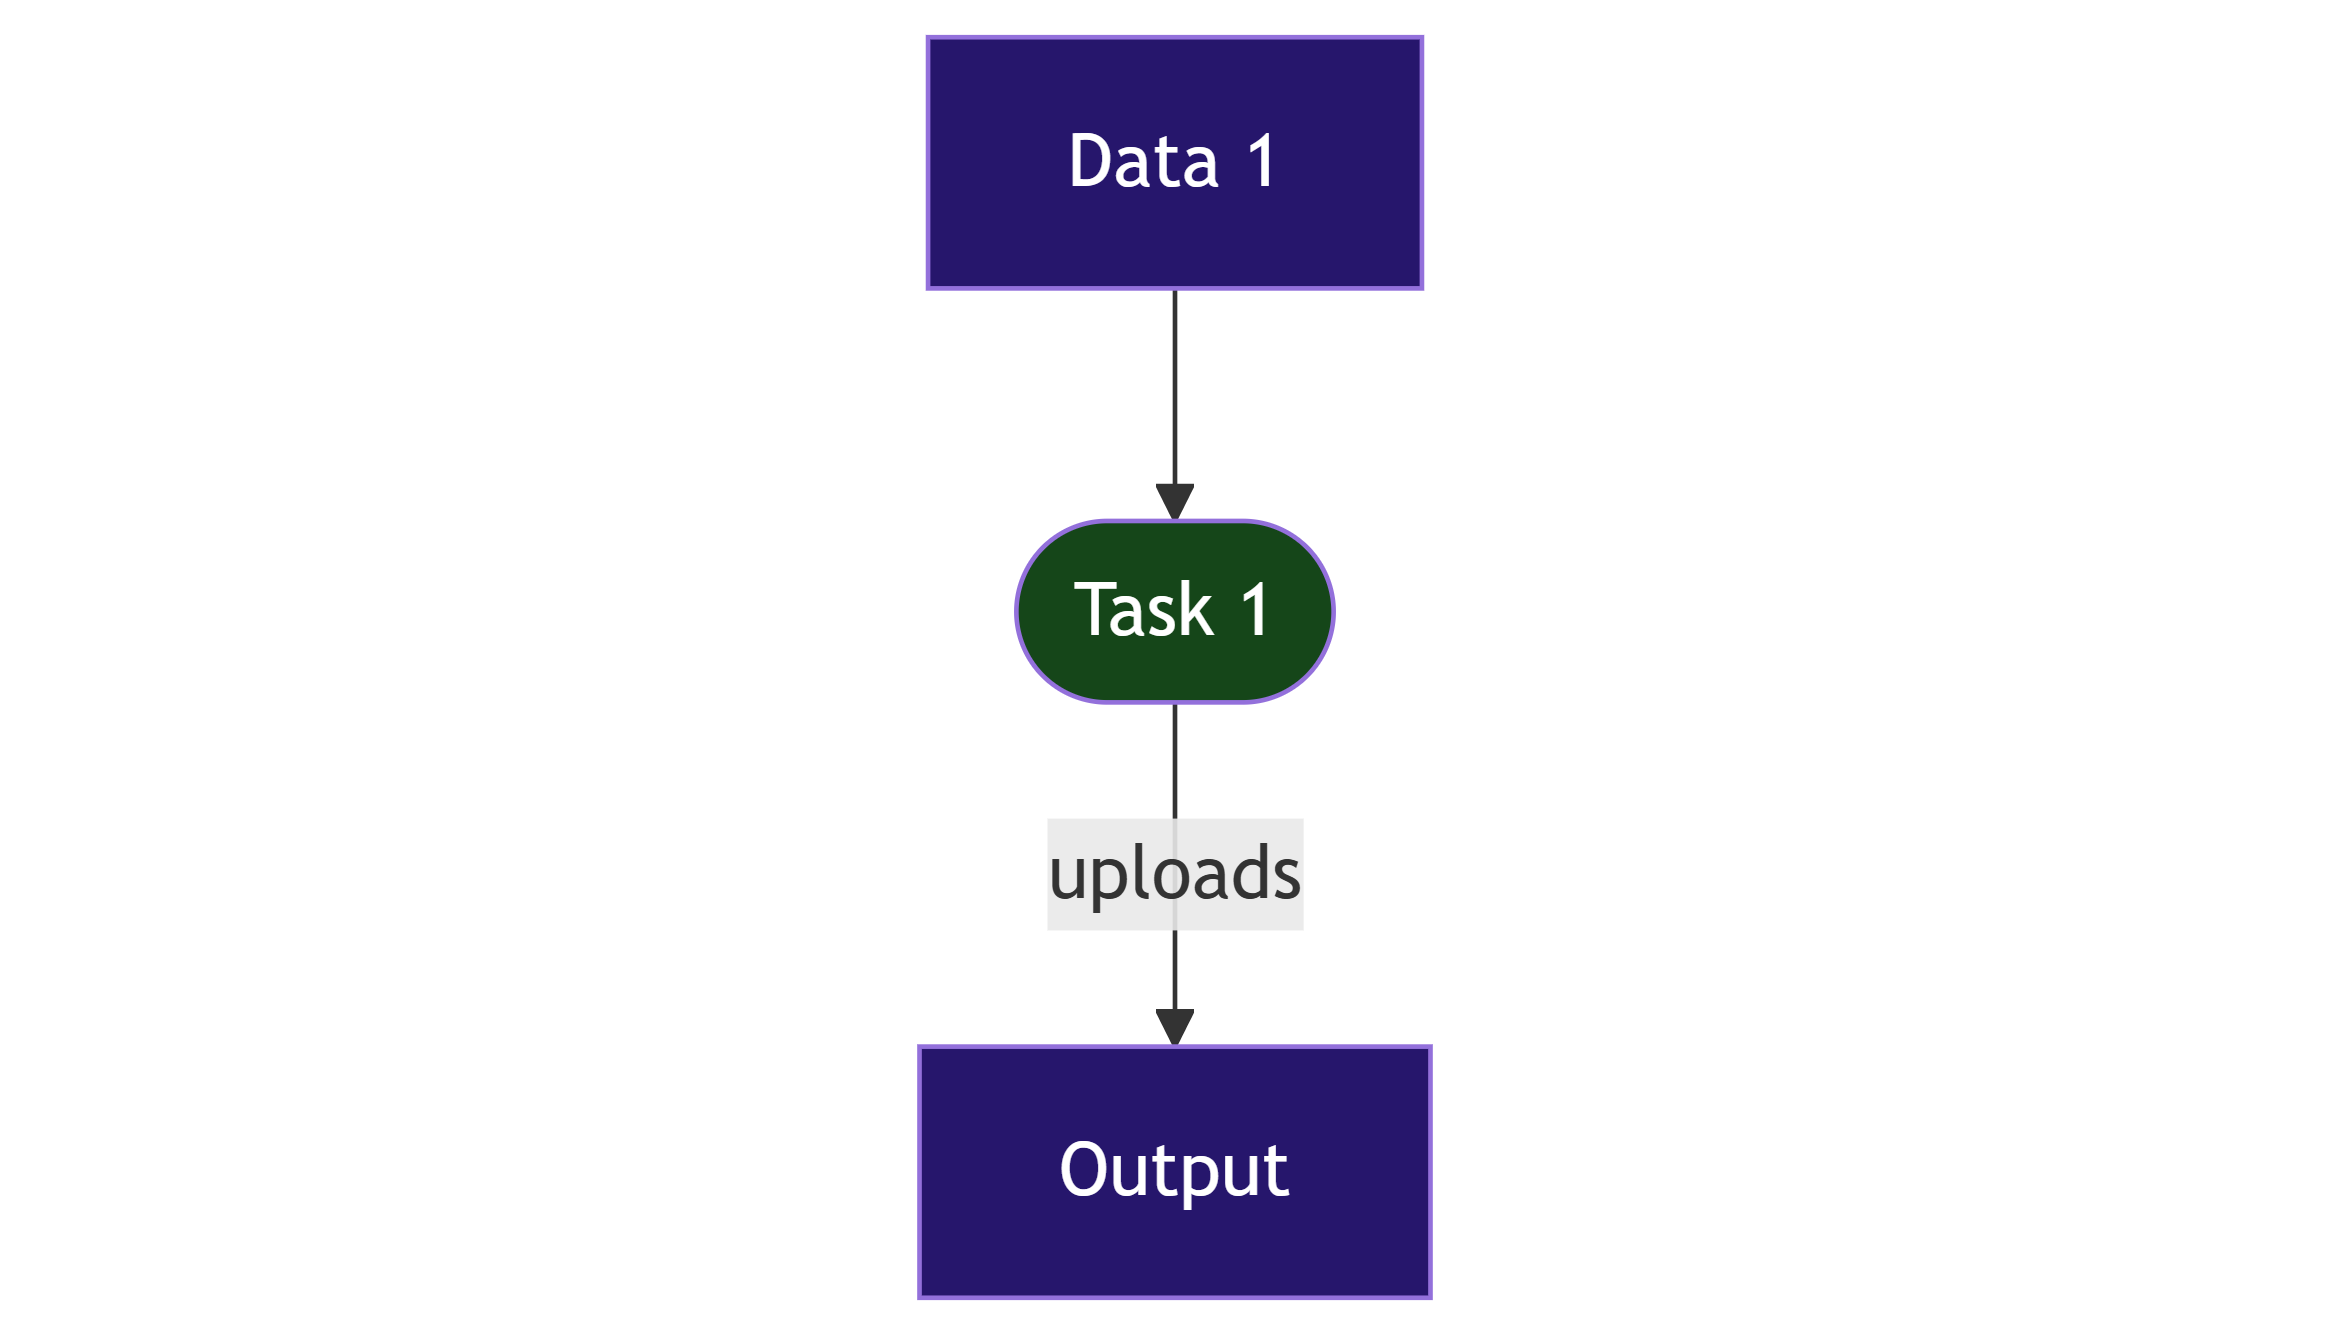
\includegraphics[width=0.95\textwidth]{mermaid-dynamic-part1.png}
      \end{column}
      \begin{column}{0.05\textwidth}
        \centering
        \vspace{1.7cm}
        \vfill
        $\Rightarrow$
      \end{column}
      \begin{column}{0.65\textwidth}
        \centering
        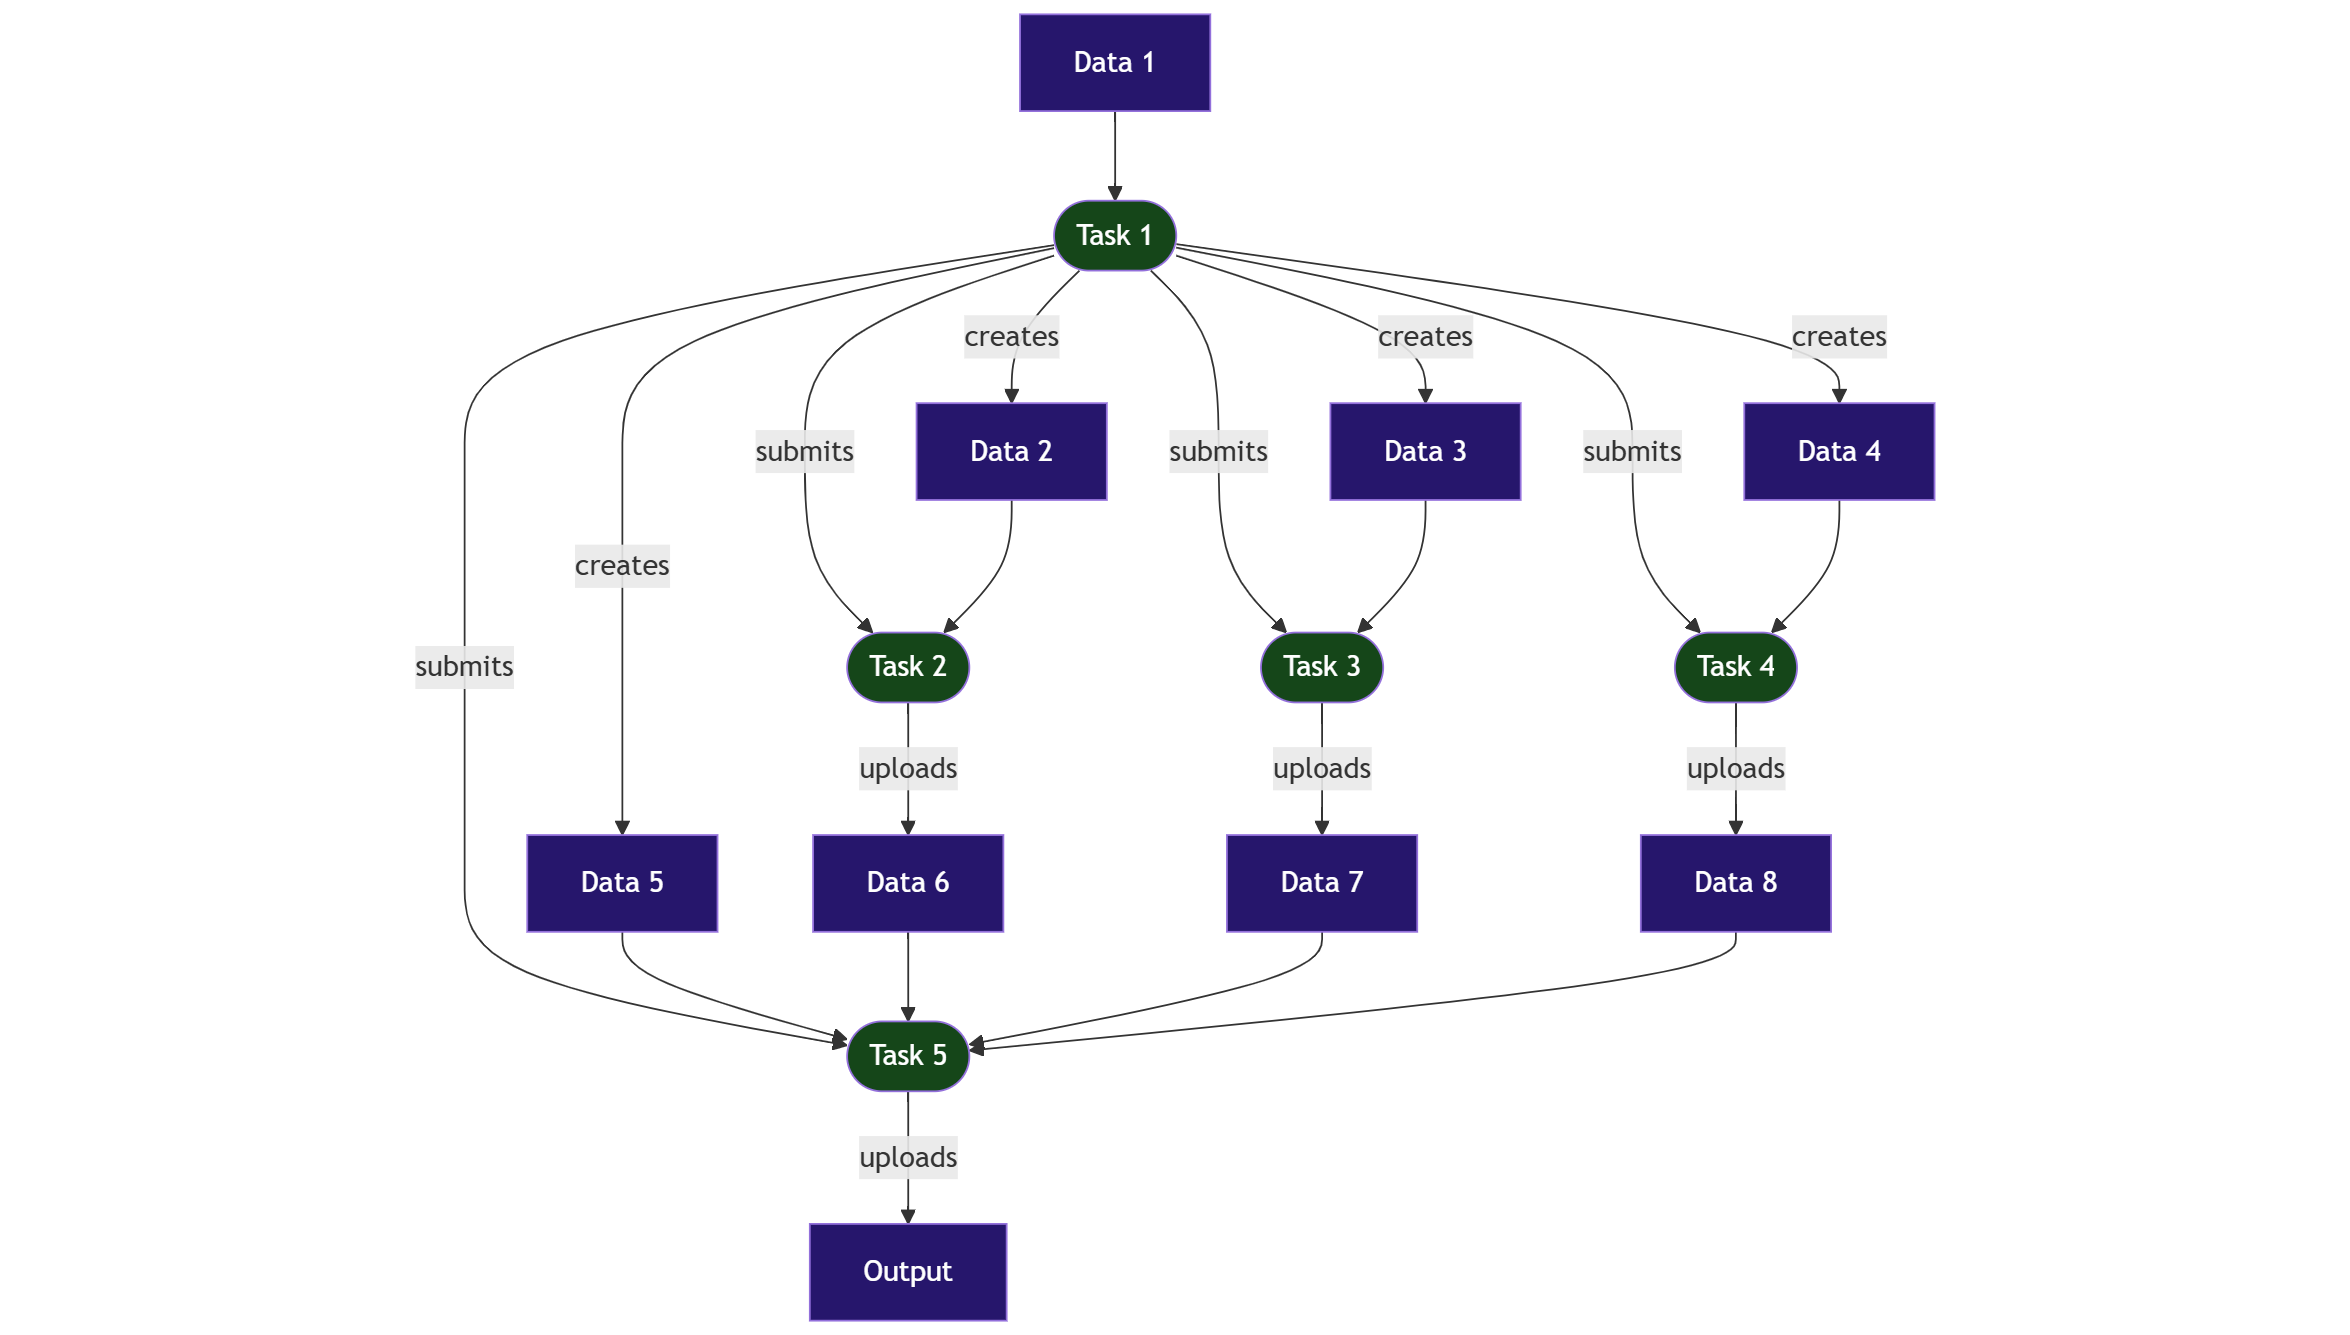
\includegraphics[width=0.95\textwidth]{mermaid-dynamic-part2.png}
      \end{column}
    \end{columns}
  \end{frame}

  \begin{frame}
    \frametitle{Data Management}
    \begin{block}{Definition}
      Responsibility for data allocation, transfer, and storage between computational operations
    \end{block}
    \begin{itemize}
      \item ArmoniK is responsible for tasks input and output data management
      \item Allows for automatic communication + scheduling/task execution overlapping
      \item Automatic Checkpointing
      \begin{itemize}
        \item Uncoordinated checkpointing for every task
      \end{itemize}
      \item Data communications through global storage
    \end{itemize}
  \end{frame}

  \begin{frame}
    \frametitle{Portability}
    \begin{block}{Definition}
      Effort to transfer an application from one environment to another
    \end{block}
    \begin{itemize}
      \item Based on container technology (Docker and Singularity)
      \item Kubernetes deployment available
      \item Cloud deployment with Managed Services
      \item Client and workers potentially available in 10+ languages with gRPC
      \begin{itemize}
        \item Officially supported: C\#, C++, Python, Rust, Java, and JavaScript
      \end{itemize}
      \item Run on x86 and ARM architectures
      \item Hybrid graphs are supported
      \begin{itemize}
        \item Tasks on different architectures, applications, environments
      \end{itemize}
      \item Supports GPU
      \item Works on Linux and Windows
    \end{itemize}
  \end{frame}

  \begin{frame}
    \frametitle{Fault Tolerance}
    \begin{block}{Definition}
      Ability to continue functioning without interruption when one or more nodes fail
    \end{block}
    \begin{itemize}
      \item Designed to support loss of all computing nodes but not all storage nodes
      \item ArmoniK internal components are stateless
      \item Status stored in high-reliability DB
      \item Error management at the task level
      \begin{itemize}
        \item Tasks retried when there are errors
        \item Manage hardware and software errors
        \item Tasks re-executed elsewhere
      \end{itemize}
      \item Allow support for preemptible computing resources
    \end{itemize}
  \end{frame}

  \begin{frame}
    \frametitle{Malleability}
    \begin{block}{Definition}
      Dynamic reconfiguration of the number of allocated resources during execution without interruption
    \end{block}
    \begin{itemize}
      \item Metrics provided to adjust computing resources to computing tasks
      \begin{itemize}
        \item Optimal number of instances to execute tasks
        \item Avoid keeping idle resources
        \item Only consume what is needed
      \end{itemize}
      \item Kubernetes autoscaling properties used
      \begin{itemize}
        \item Could be swapped with another resource manager/allocator
      \end{itemize}
    \end{itemize}
  \end{frame}

  \begin{frame}
    \frametitle{Resource Sharing}
    \begin{block}{Definition}
      Share resources between applications
    \end{block}
    \begin{itemize}
      \item Scheduling multiple applications at the same time on the same resources
      \item Resources only used when needed
      \item Leverage maximum task parallelism
      \item Maximizing tasks throughput, not minimizing latency
    \end{itemize}
  \end{frame}

  \begin{frame}
    \frametitle{Modularity}
    \begin{block}{Definition}
      Modules can be swapped without modifying ArmoniK's code
    \end{block}
    \begin{itemize}
      \item \textbf{Containers}:
      \begin{itemize}
        \item Can be executed everywhere container runtime is available
        \item Not easy, but difficulty is manageable
      \end{itemize}
      \item \textbf{Queue system}:
      \begin{itemize}
        \item Manages task execution ordering and distribution
        \item Interface is provided, and plugins can be loaded dynamically
        \item Allows swapping for another queue system or orchestration strategy
      \end{itemize}
      \item \textbf{Object storage}:
      \begin{itemize}
        \item Manages data storage in ArmoniK (tasks input and output)
        \item Interface is provided, and plugins can be loaded dynamically
        \item Allows storing data where the user wants/needs
      \end{itemize}
    \end{itemize}
  \end{frame}

  \begin{frame}
    \frametitle{Observability}
    \begin{block}{Definition}
      Ability to understand the internal state of a system based solely on its external outputs.
    \end{block}
    \begin{itemize}
      \item GUI to monitor workflows and tasks status (optional)
      \item Expose metrics about ArmoniK and tasks states
      \item Tooling to emit, collect and search application/orchestration logs
      \item Provide monitoring APIs that can show tasks and data status
      \begin{itemize}
        \item Available in multiple languages
        \item Can be integrated into monitoring systems
      \end{itemize}
      \item CLI built on top of our APIs
      \begin{itemize}
        \item Can be improved to support more features
        \item We are open to suggestions
      \end{itemize}
    \end{itemize}
  \end{frame}

  \begin{frame}
    \frametitle{Production-ready}
    \begin{block}{Definition}
      System that meets all functional and non-functional requirements, is thoroughly tested, and is stable, secure, scalable, and maintainable enough to be deployed in a live production environment.
    \end{block}
    \begin{itemize}
      \item In production!
      \item Used by clients for their critical computations
      \item Explains our needs for:
      \begin{itemize}
        \item Validation and guarantees
        \item Monitoring
        \item Stability
      \end{itemize}
    \end{itemize}
  \end{frame}

\end{section}

\begin{section}{How we plan to adress larger scale applications ?}
  \begin{frame}
    \frametitle{Data Management Optimization}
    \begin{itemize}
      \item As of today, every data is read and written from our object storage
      \begin{itemize}
        \item Even in the case the data was used or produced in the preceding task
        \item Ensures no data loss
        \item Very costly and sub-optimal
      \end{itemize}
      \item Optimizations
      \begin{itemize}
        \item Node-level caching system
        \item P2P Distributed storage system to harness RDMA performances
        \item Checkpointing strategies
      \end{itemize}
    \end{itemize}
  \end{frame}

  \begin{frame}
    \frametitle{Data-Aware Scheduling Strategies}
    \begin{itemize}
      \item Current scheduling
      \begin{itemize}
        \item Dependencies resolution managed by ArmoniK
        \item Tasks distribution done by the queue system (contains only tasks with dependencies available)
      \end{itemize}
      \item Improvements
      \begin{itemize}
        \item Affinity task-data
        \begin{itemize}
          \item Schedule tasks to the agent where inputs are in cache or close
          \item Colocate sub-graphs with common dependencies
        \end{itemize}
        \item Fine-grained data lifecycle management
        \begin{itemize}
          \item Data usage hints to help remove data from cache when not used anymore
          \item Data can be used as dependencies during new tasks submission (dynamic graph)
          \item Help scheduler during task distribution
        \end{itemize}
      \end{itemize}
    \end{itemize}
  \end{frame}

  \begin{frame}
    \frametitle{Supercomputer Deployment}
    \begin{itemize}
      \item Kubernetes not available on most supercomputers
      \item Needs an alternative resource manager for ArmoniK
      \begin{itemize}
        \item Run ArmoniK within a SLURM job
        \item More advanced integration with SLURM
        \begin{itemize}
          \item Use SLURM as ArmoniK resource manager
          \item Take advantage of SLURM queues to run ArmoniK compute plane
        \end{itemize}
      \end{itemize}
      \item Docker not available too
      \begin{itemize}
        \item Docker rootless
        \item Singularity
      \end{itemize}
      \item Need tests and integration in order to validate it works properly
      \item Done by HPC-Whisk
    \end{itemize}
  \end{frame}

  \begin{frame}
    \frametitle{Federation}
    \begin{block}{Definition}
      Manage and use multiple ArmoniK instances as one
    \end{block}
    \begin{itemize}
      \item Multi-site deployment
      \begin{itemize}
        \item Multiple instances on the same cloud provider
        \item Different cloud
        \item On-prem and cloud
      \end{itemize}
      \item Load balancing
      \begin{itemize}
        \item Choose the best instance according to usage, price, data sensitivity, arbitrary data, etc.
        \item Allow users to implement their own policies
      \end{itemize}
      \item Bursting
      \begin{itemize}
        \item When/How to split the graph?
        \item How to avoid/reduce data migration between two instances?
      \end{itemize}
    \end{itemize}
  \end{frame}

  \begin{frame}
    \frametitle{Performance Analysis Tools}
    \begin{itemize}
      \item Usually a complex task due to the complexity of the problem solved and the software stack
      \item Increased complexity with ArmoniK's malleability making the number of resources used vary
      \item Provide data usable for performance analysis
      \item Build tooling to allow users to easily identify performance bottlenecks
    \end{itemize}
  \end{frame}

  \begin{frame}
    \frametitle{Hybrid Computations Use Cases}
    \begin{itemize}
      \item Coupling HPC application and ArmoniK applications
      \begin{itemize}
        \item HPC code is ArmoniK's client
      \end{itemize}
      \item HPC workloads
      \begin{itemize}
        \item ArmoniK is used to implement the whole application
      \end{itemize}
      \item Application mixing CPU/GPU/QPU
    \end{itemize}
  \end{frame}

  \begin{frame}
    \frametitle{Formal Validation of ArmoniK's Properties}
    \begin{itemize}
      \item Quentin's PhD goal
      \item Modelize ArmoniK scheduler
      \item Validate scheduling is fault tolerant, efficient, and malleable
    \end{itemize}
  \end{frame}
\end{section}

\begin{section}{Are you interested in our solution ? $\rightarrow$ Come next session}
  \begin{frame}
    \frametitle{Open source project}
    \begin{itemize}
      \item ArmoniK code is fully available on github
      \item \href{https://github.com/aneoconsulting/ArmoniK}{ArmoniK's GitHub}
      \item You can contribute
      \item We are open to collaborations
      \item How to use it ?
      \begin{itemize}
        \item \href{https://armonik.readthedocs.io/en/latest/content/armonik/getting-started.html}{Getting started}
      \end{itemize}
    \end{itemize}
  \end{frame}

  \begin{frame}
    \frametitle{Next session}

    Come use ArmoniK with us!

  \end{frame}

  \begin{frame}
    \frametitle{Thank you for your attention!}
    Questions?
  \end{frame}
\end{section}

\end{document}